% Ejemplo de documento LaTeX
% Tipo de documento y tamaño de letra
\documentclass[12pt]{article}


\usepackage[spanish]{babel}
\usepackage{longtable} 
\selectlanguage{spanish}
\usepackage[utf8x]{inputenc}
\usepackage{graphicx}




% EL titulo, autor y fecha del documento
\title{Reporte de Actividad 4}
\author{Carlos Medina}
\date{27-2-15}


% Aqui comienza el cuerpo del documento
\begin{document}
% Construye el título
\maketitle


El siguiente reporte describirá los pasos realizados para la actividad 4 (2015-1), así como se mostrarán los resultados de ésta.




\hspace {0.5cm} En matemáticas, una serie de Taylor o polinomio de Taylor es una representación de una funcion como una suma infinita de términos que son calculados por los valores de las derivadas de la funcion en un solo punto.

El concepto de una serie de Taylor fue descubierta por el matemático escocés James Gregory y formalmente introducido por el matemático ingles Brook Taylor en 1715. Si las series de Taylor se centran en cero, entonces se les llama también "Polinomio de Maclaurin", nombrados después de que el matemático escocés Colin Maclaurin, uso un extenso uso de este caso especial de la serie de Taylor en el siglo XVIII.


La serie de Taylor de una función f real o compleja f(x) infinitamente diferenciable en el entorno de un número real o complejo a es la siguiente serie de potencias:

\begin{center}
	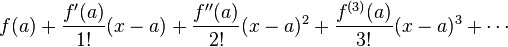
\includegraphics[width=13cm]{Tay.png}\\
\end{center}

que puede ser escrito de una manera más compacta como la siguiente sumatoria:

\begin{center}
	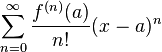
\includegraphics[width=4cm]{Taysum.png}\\
\end{center}


Donde n! es el factorial de n, f(n)(a) denota la n-ésima derivada de f para el valor a de la variable respecto de la cual se deriva.
La derivada de orden cero de f es definida como la propia f y tanto (x − a)0 como 0! son ambos definidos como 1 (0! = 1). En caso de ser a = 0, como ya se mencionó, la serie se denomina también de MacLaurin.

En la siguiente actividad graficaremos con una herramienta de linux muy útil en el ámbito profesional y amateur de los científicos, Gnuplot.

Gnuplot es un programa muy flexible para generar gráficas de funciones y datos. Este programa es compatible con los sistemas operativos más populares (Linux, UNIX, Windows, Mac OS X...). El origen de gnuplot data de 1986.

Gnuplot puede producir sus resultados directamente en pantalla, así como en multitud de formatos de imagen, como PNG, EPS, SVG, JPEG, etc. Se puede usar interactivamente o en modo por lotes (batch), usando scripts. Este programa tiene gran base de usuarios y está convenientemente mantenido por sus desarrolladores. Existe una ingente cantidad de ayuda en Internet, aunque gran parte está en inglés.

\vspace {0.5cm}

\hspace {0.5cm} A continuación veremos unos ejemplos de cómo calcular estos polinomios en la herramienta $Gnuplot$, desde $Maxima$.

\vspace {0.5cm} Primero se pide reproducir exactamente la gráfica de la aproximación de Taylor de la función sen(x), de aproximación 1, 3, 5 y 7. Esto se grafica con el código:
     
     \begin{verbatim}
     
  f(x):= sin(x);
T1(x):=taylor(f(x), x, 0, 1);
T3(x):=taylor(f(x), x, 0, 3);
T5(x):=taylor(f(x), x, 0, 5);
T7(x):=taylor(f(x), x, 0, 7);
fortran(T1(x));
fortran(T3(x));
fortran(T5(x));
fortran(T7(x));
tex(T1(x));
tex(T3(x));
tex(T5(x));
tex(T7(x));
plot2d ([f(x),T1(x), T3(x), T5(x), T7(x)], [x, -%pi, %pi], [y, -2, 2], 
[color,blue,orange,red,black,green],[legend, "f", "P1", "P3", "P5", "P7"],       
[axes, true], [ylabel,"sin(x)"]); 
    
     \end{verbatim}
     
Después, $Maxima$ lo grafica los varios polinomios que agregamos en el código, quedándonos de la siguiente manera:

\begin{center}
	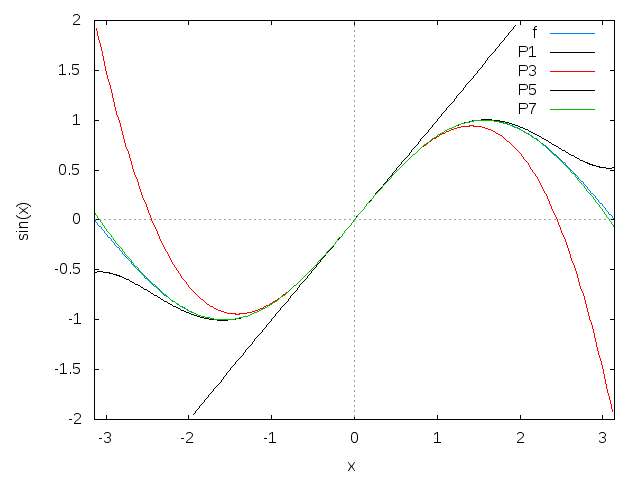
\includegraphics[width=15cm]{Sen.png}\\
\end{center}

Como se pruede observar, mientras más grande es el grado del polinomio, más se parece a la función. Se señala con P1, P3, P5 y P7 a las curvas que describe cada polinomio con su respectivo grado.

Ahora se pide ahora obtener la aproximación de Taylor de la función log(1+x), para las aproximaciones de grado 4, 7, 11 y 16. Modificamos el código y nos quedará de la siguiente forma:

\begin{verbatim}
f(x):= log(1+x);
T4(x):=taylor(f(x), x, 0, 4);
T7(x):=taylor(f(x), x, 0, 7);
T11(x):=taylor(f(x), x, 0, 11);
T16(x):=taylor(f(x), x, 0, 16);
fortran(T4(x));
fortran(T7(x));
fortran(T11(x));
fortran(T16(x));
tex(T4(x));
tex(T7(x));
tex(T11(x));
tex(T16(x));
plot2d ([f(x),T4(x), T7(x), T11(x), T16(x)], [x, -1.5, 1.5], [y, -4, 2], 
[color,pink,green,red,orange,blue],[legend, "log(1+x)", "P4", "P7", "P11",
 "P16"],[axes, true], [ylabel,"log(1+x)"]);
\end{verbatim}

Esto nos graficará y nos mostrará la siguiente gráfica:

\begin{center}
	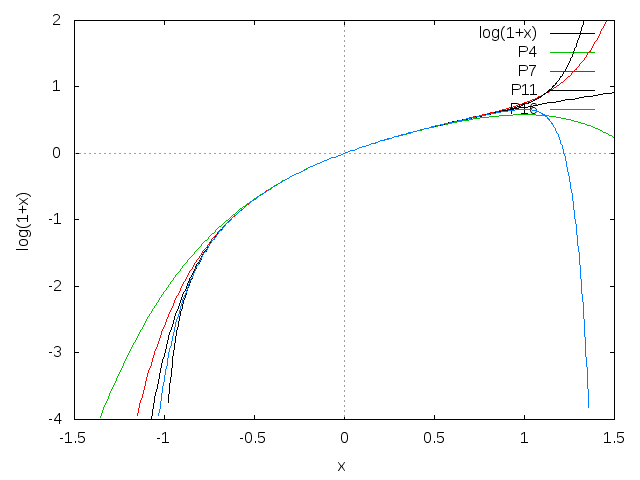
\includegraphics[width=15cm]{Log.png}\\
\end{center}

Ahora, de la misma forma, se calcula la aproximación de la serie de Taylor de la función log(cos(x)), alrededor del punto  x=0, en el rango (-pi/2, pi/2), usando polinomios de varios grados, los cuales elegimos a nuestro gusto. El código se escribe, modificando el rango como se pide, y quedará de la siguiente manera:

\begin{verbatim}
f(x):= log(cos(x));
T2(x):=taylor(f(x), x, 0, 2);
T7(x):=taylor(f(x), x, 0, 7);
T11(x):=taylor(f(x), x, 0, 11);
T16(x):=taylor(f(x), x, 0, 16);
fortran(T2(x));
fortran(T7(x));
fortran(T11(x));
fortran(T16(x));
tex(T2(x));
tex(T7(x));
tex(T11(x));
tex(T16(x));
plot2d ([f(x),T2(x), T7(x), T11(x), T16(x)], , [color,pink,green,red,orange,blue],[legend, "log(cos(x))", "P2", "P7", "P11", "P16"],[axes, true], [ylabel,"log(cos(x))"]);
\end{verbatim}

Se puede observar que cambiamos el rango en la sección para realizar la gráfica con los márgenes como se piden. Se muestra lo dicho en la imagen:

\begin{center}
	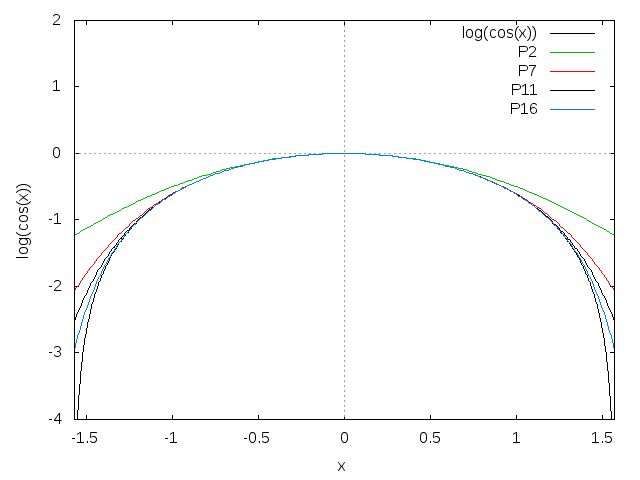
\includegraphics[width=15cm]{LogCos.png}\\
\end{center}

Ahora, calcularemos las aproximaciones de Taylor de la función exp(x)/cos(x), alrededor de x=0. Para esto no es necesario modificar tantos valores, con sólo cambiar la función anterior por la que se nos pide, quedándonos con:

\begin{verbatim}
f(x):= exp(x)/cos(x);
T2(x):=taylor(f(x), x, 0, 2);
T7(x):=taylor(f(x), x, 0, 7);
T11(x):=taylor(f(x), x, 0, 11);
T16(x):=taylor(f(x), x, 0, 16);
fortran(T2(x));
fortran(T7(x));
fortran(T11(x));
fortran(T16(x));
tex(T2(x));
tex(T7(x));
tex(T11(x));
tex(T16(x));
plot2d ([f(x),T2(x), T7(x), T11(x), T16(x)], [x, -%pi/2, %pi/2], [y, 0, 2], [color,pink,green,red,orange,blue],[legend, "exp(x)/cos(x)", "P2", "P7", "P11", "P16"],[axes, true], [ylabel,"exp(x)/cos(x)"]);
\end{verbatim}

\begin{center}
	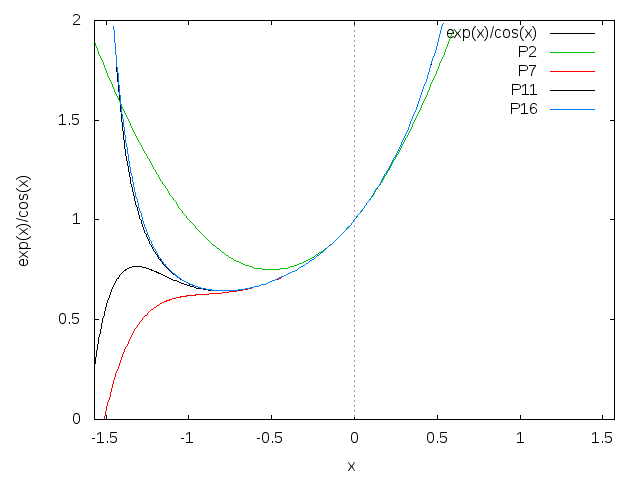
\includegraphics[width=15cm]{ExpCos.png}\\
\end{center}

Por último, de la misma forma, ejemplificamos la aproximación de Taylor de la función (1+x) exp(x), alrededor de x=0. Se puede notar el asterisco agregado en medio de las funciones (1+x) y exp(x), significa que se multiplican, ya que Maxima no distingue multiplicaciónes con paréntesis.

\begin{verbatim}
f(x):= (1+x)*exp(x);
T2(x):=taylor(f(x), x, 0, 2);
T7(x):=taylor(f(x), x, 0, 7);
T11(x):=taylor(f(x), x, 0, 11);
T16(x):=taylor(f(x), x, 0, 16);
fortran(T2(x));
fortran(T7(x));
fortran(T11(x));
fortran(T16(x));
tex(T2(x));
tex(T7(x));
tex(T11(x));
tex(T16(x));
plot2d ([f(x),T2(x), T7(x), T11(x), T16(x)], [x, -6, 2], [y, -2, 6], [color,pink,green,red,orange,blue],[legend, "(1+x)*exp(x)", "P2", "P7", "P11", "P16"],[axes, true], [ylabel,"(1+x)*exp(x)"]);
\end{verbatim}

Y se muestra en la gráfica siguiente:

\begin{center}
	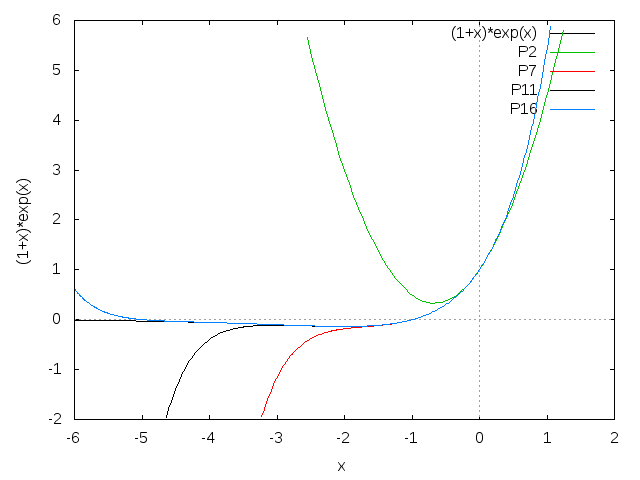
\includegraphics[width=15cm]{Exp1.png}\\
\end{center}

Como vimos en este reporte, los polinomios de Taylor sirven de mucho ya que son una forma más acertada de aproximar una función, dependiendo del grado que utilices. También aprendimos que Gnuplot es una herramienta muy efectiva graficando funciones, y, en este caso, polinomios de Taylor, viéndose claramente los resultados.

% Nunca debe faltar esta última linea.
\end{document}
